\documentclass{article}

\title{Flow-induced shape reconfiguration in houseplants}
\author{C Smith}
\date{\today}

\usepackage{siunitx}
\usepackage{graphicx}
\usepackage[round,authoryear]{natbib}
\bibliographystyle{apalike}
\usepackage[plain]{fancyref}
\usepackage{listings}
\lstset{
  basicstyle=\ttfamily}
\usepackage{amsmath,amsfonts,amssymb}
\usepackage{booktabs}

\begin{document}
\maketitle
\begin{abstract}
This study was conducted to investigate how effectively citrus plants can change their structure to generate less drag in wind. A cord with known spring constant was attached to a young grapefruit plant and an aluminum model of one of its leaves, a box fan was used to create a wind tunnel, and area was calculated using Matlab's color thresholding and blob detection software. The actual drag created on the grapefruit leaves was significantly less than the drag expected on an identical model, and slow motion video analysis indicated that this was the result of the citrus's ability to bend at the petiole. The extreme bending in several directions showed the plant's inclination toward protective load shedding.

\end{abstract}

\section{Introduction}
%Smith: The main ones to look at closely are Vogel and also Laura Miller and Company, and then the algae stuff from Emily Carrington, Mark Denny, Hannah Stewart, etc. May also search on ecological safety factors, reconfigurable structures, use of physical models. I didn't check mangrove literature for drag and shape reconfiguration, I think there's also coral literature about corals breaking during hurricanes to reduce loads / save the colony from death. In engineering context, this is same idea as protective load shedding in electrical systems, or crumple zones and holding bulkheads in structural systems; reefing during sailing, etc. 

Work from an inverted triangle (broader topics to more specific). Explain what you are interested, review some relevant literature, and then set up what your specific research question is. Cite literature using the author-year format, as in \citep{buck2020go}. If you need pictures to explain the relevant biomechanics, feel free to include. This section should also say a little why your research matters. 
% things to explain include drag, how it depends on speed, area, etc; why it matters to plants, what they can do to minimize or mitigate drag...
The last part of this section should be the specific hypotheses you seek to test. 

\section{Methods and materials}
\begin{itemize}
\item 1 six-year old grapefruit plant
\item 1 cord of known spring constant
\item 1 measuring tape
\item 1 Kaz Inc. Ht-908 15 inch Honeywell Turbo Force Room Air Circulator Fan
\item colored construction paper
\item 1 pair of scissors
\item clear tape
\item 1 Samsung Galaxy S-8 smartphone camera
\item 1 wooden chair
\item flat, rectangular surfaces
\item MATLAB software
\item pipe cleaners
\item nylon rope
\end{itemize}

The first step in the process was to find a cord of known spring constant. In this experiment, a cord from a party mask was found to have a spring coefficient of 0.589 lbf/in. The cord was attached to a nylon rope and tied to pipe cleaners at both ends so that it could be connected to plant stems. The pipe cleaners were included in the spring constant calculation.

The experimental setup for measuring the spring's deflection due to drag is shown in Figure 1. The cord was strung between a heavy chair and the trunk of a grapefruit plant so that it was not slack, and its length was measured using a tape measure. Then, a box fan was placed one foot away from the trunk of the plant. The plant and fan were raised using flat, rectangular objects, such as textbooks, in order to position the plant's canopy in front of the fan. The cord's deflection was measured five times at each of the fan's three speed settings and a slow motion video of the plant's leaves was taken at the highest fan setting.

Next, the cross sectional area of the plant was calculated using color blob detection in Matlab. To do this, black construction paper was cut to the size and shape of the fan's opening and affixed to it. Because air was blowing from relatively close to the plant, only the area which was directly in front of the fan opening would be exposed to wind. The plant was of a complex shape, so it was more efficient to calculate the area of the fan which was not covered by the plant. The setup was photographed from afar and scaled to eliminate the colorful surroundings, as shown in Figure 2. A picture of the fan-shaped paper was also taken against a blue background from the same distance with no citrus obscuring it and scaled by the same amount, which can also be seen in Figure 2. Using Matlab's colorThresholder system, the ratio of covered to uncovered area was found and multiplied by the known paper area to find the area of the grapefruit leaves.

After analyzing the results of the grapefruit plant, a rigid model was created to test the same conditions without the presence of bending. A small leaf was placed against an aluminum Chipotle bowl lid to serve as a stencil, which was cut out using scissors. Then, this model leaf was taped to a wooden pencil so that the pencil would prevent it from flexing, while any tape edges were cut off. The finished leaf model can be seen in 
Figure 3.

The leaf model was tested in the same manner as the grapefruit plant at the highest fan setting. Because the deflection in the cord was quite small, the displacement was measured using slow motion video. To do this, a tape measure with millimeters marked was taped below the cord and the video was taken from directly above. The video device was planted on a solid surface to minimize movement, and the displacement was found by zooming in on the video and pausing when the cord was fully extended and relaxed. 

In order to compare the model area to the area of the grapefruit, a sheet of orange construction paper was photographed with and without the model leaf against it. Then, using the color blob detection technique in Matlab, the ratio of the model area to the paper area was calculated and multiplied by the actual paper area, in square feet. The images for this analysis can be seen in Figure 4.

With the approximate cross sectional areas of the actual grapefruit leaves and the model found, the discussion over how these areas and their corresponding drags differed could begin.


% Fig 1 is good but cluttered, can we zoom in on only the business part; or turn it into a drawing. Altnatively, add callouts and scale bar? Is there a shot more from the side, that shows the experimental rig without foreshortening? 
\begin{figure}
\begin{center}
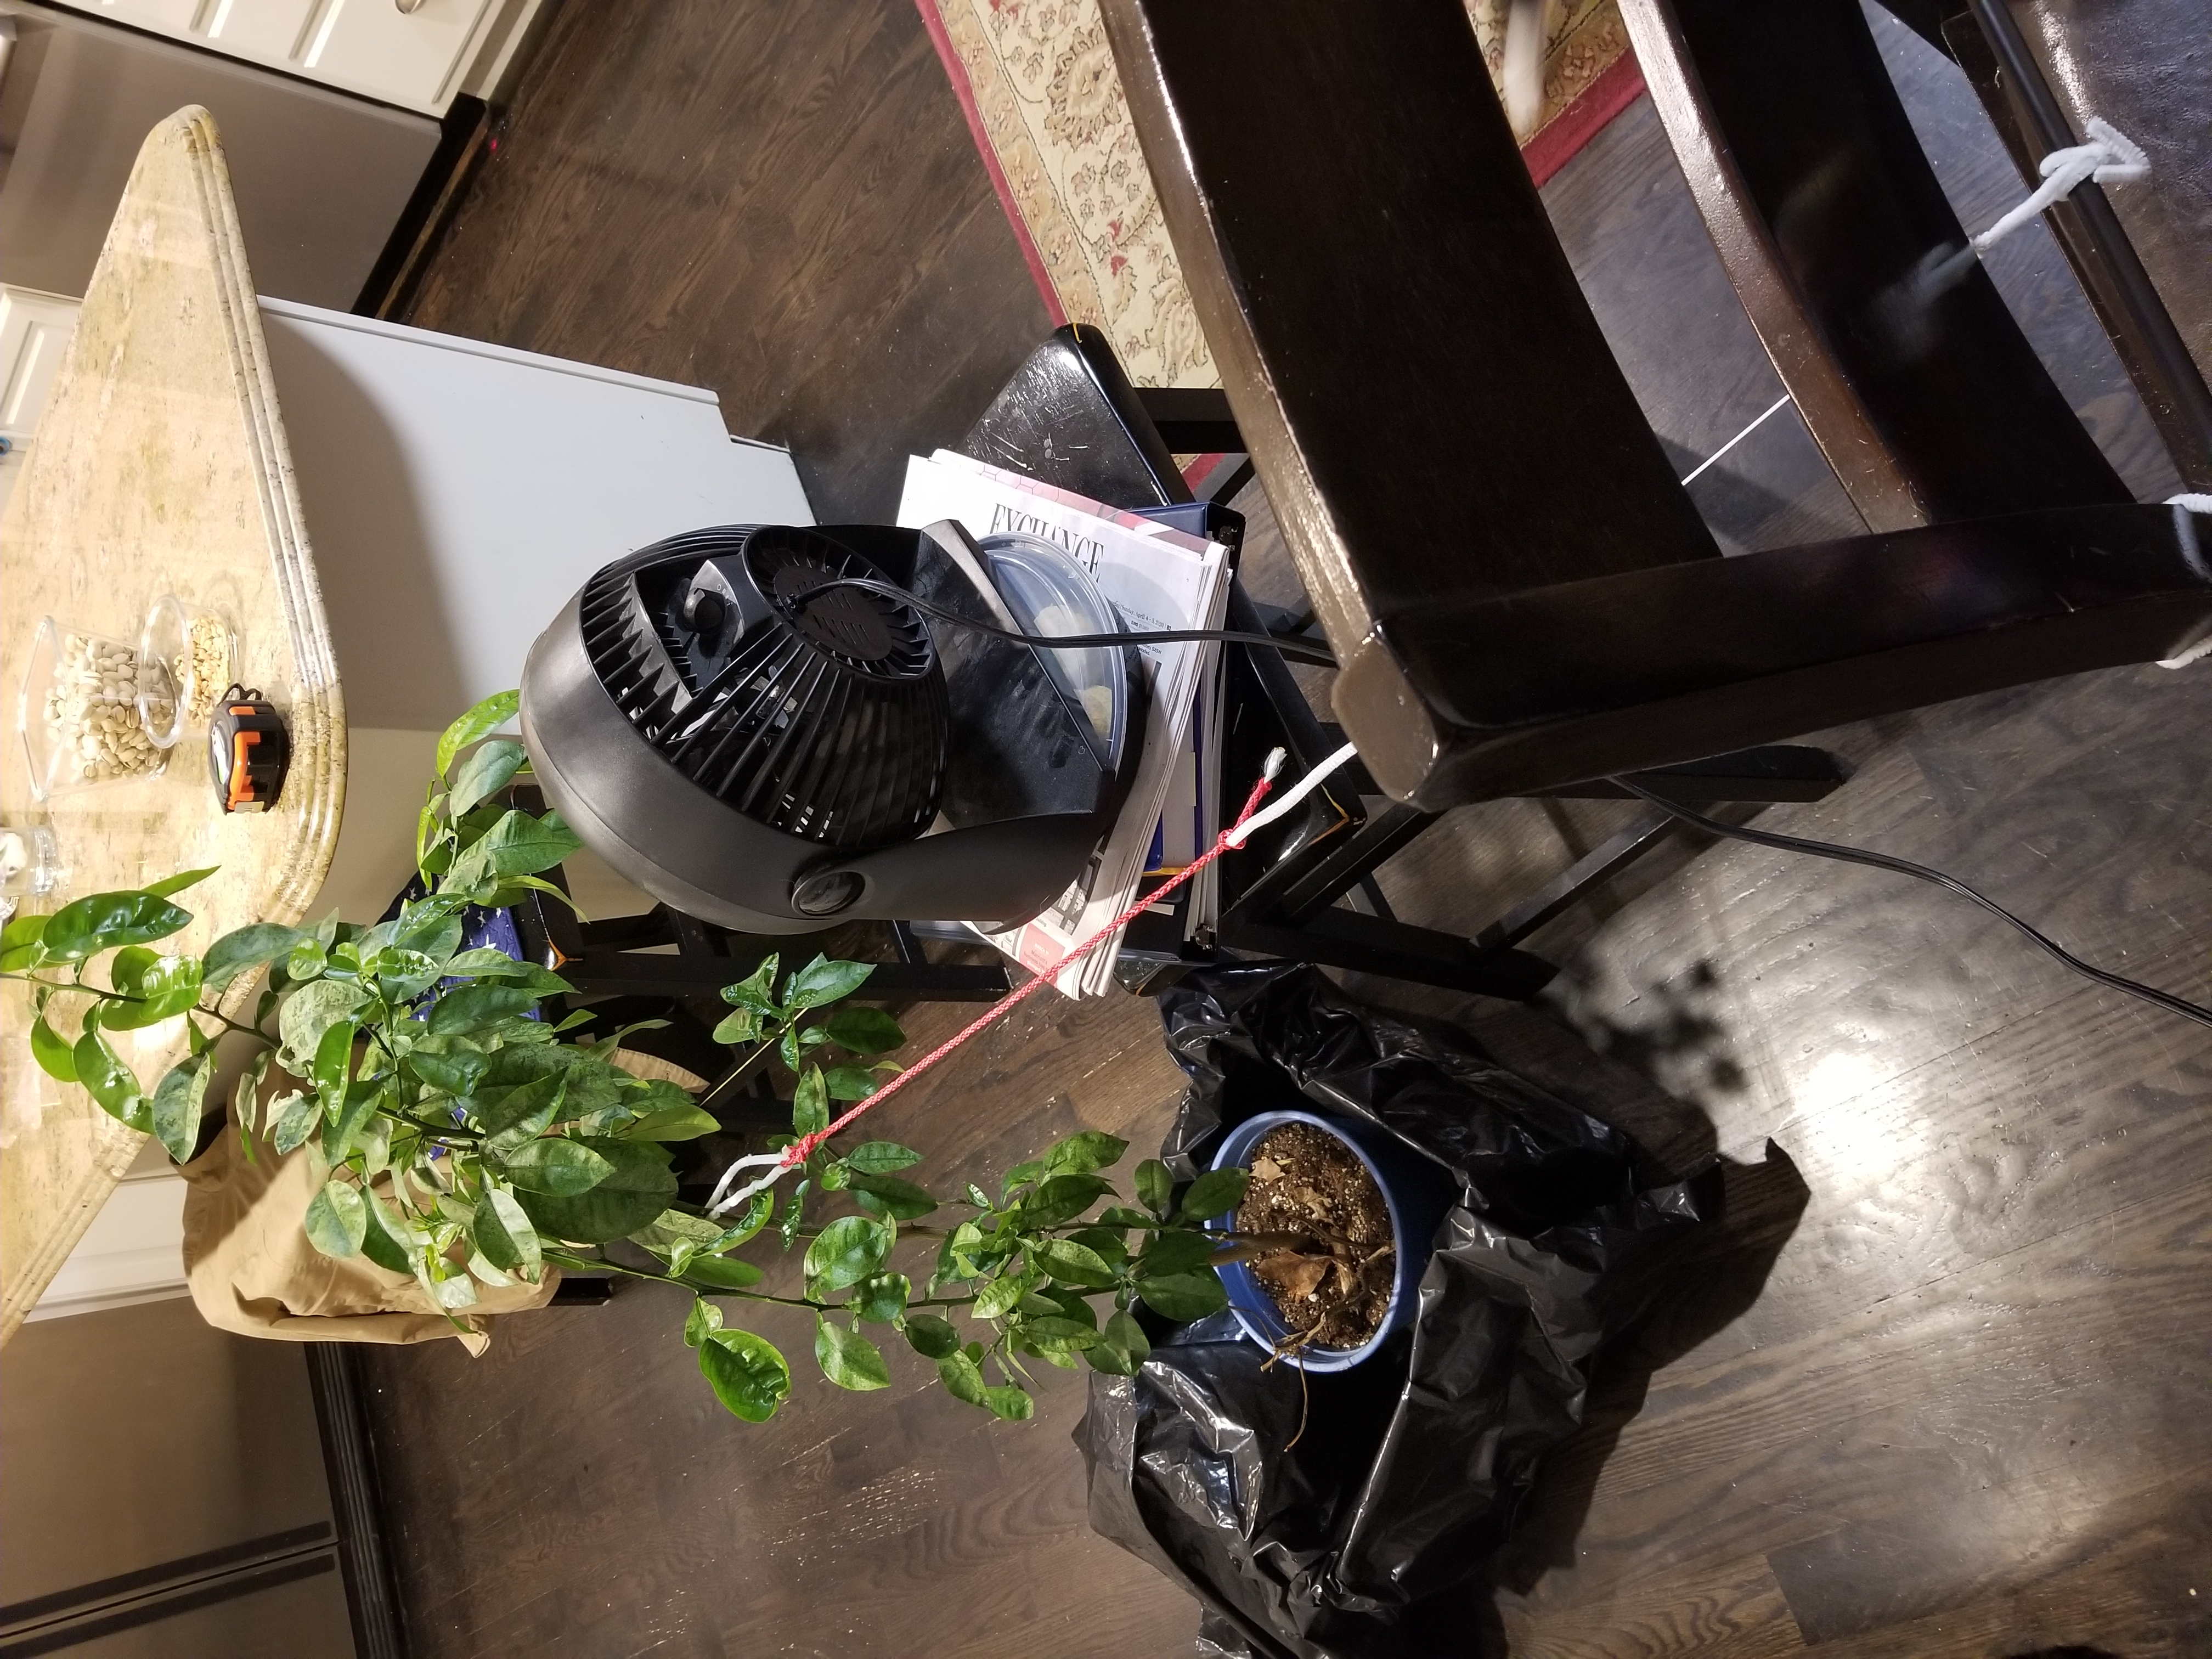
\includegraphics[width=0.5\columnwidth]{Grapefruit_Setup.jpg} 
\end{center}
\caption{Experimental setup to measure the deflection of a grapefruit plant when exposed to wind.}
\label{fig:methods1}
\end{figure}

% Not sure what you get from Fig 2; I might move it to appendix. 
\begin{figure}
\begin{center}
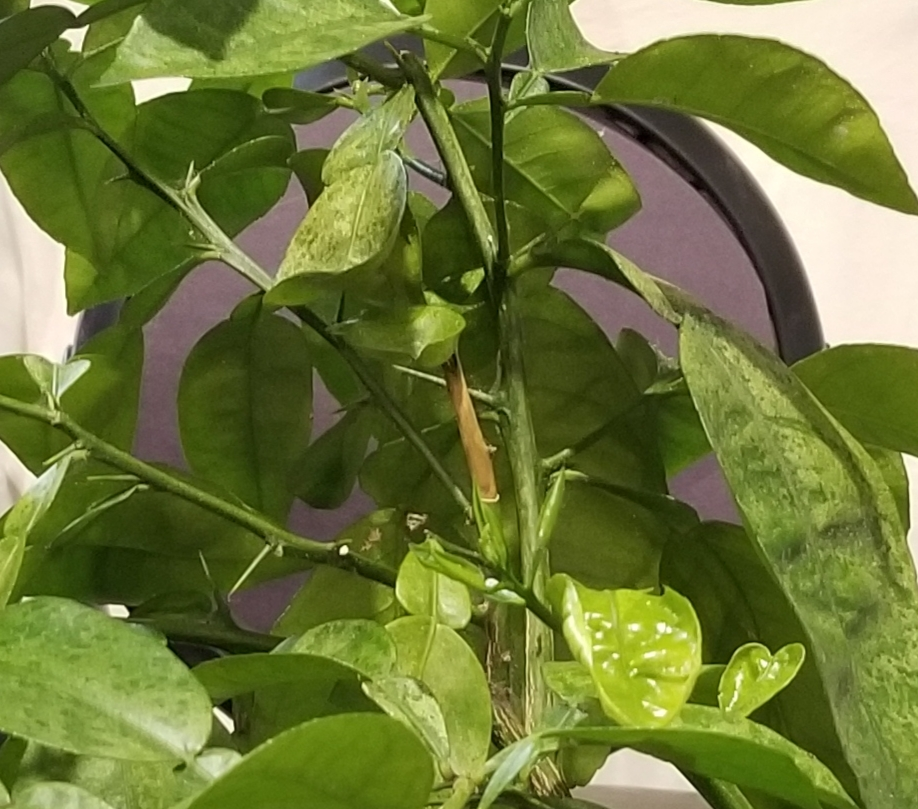
\includegraphics[width=0.33\columnwidth]{Fan.jpg}
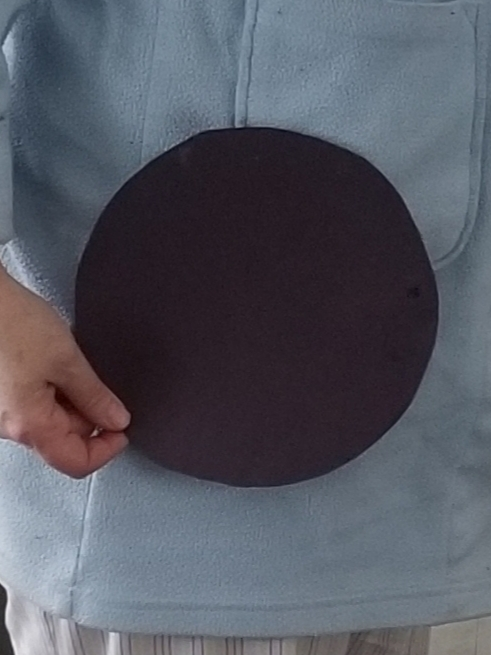
\includegraphics[width=0.33\columnwidth]{Fan1.jpg}
\end{center}
\caption{The exposed area of the fan-shaped construction paper with and without the plant in front of it.}
\label{fig:methods2}
\end{figure}

% Fig 3 is good but zoom in on the two, add callouts and a scalebar, maybe rotate leafs into their normal positions. 
\begin{figure}
\begin{center}
\includegraphics[width=0.5\columnwidth]{Metal_Leaf_Compared.jpg}
\end{center}
\caption{The aluminum grapefruit leaf model (right) with a small jackfruit leaf, for scale.}
\label{fig:methods3}
\end{figure}

% Not sure what Fig 4 adds, might move to appendix. 
\begin{figure}
\begin{center}
\includegraphics[width=0.33\columnwidth]{MetalLeaf.jpg}
\includegraphics[width=0.33\columnwidth]{Paper.jpg}
\end{center}
\caption{The orange construction paper of known area photographed with and without the model leaf overlaid.}
\label{fig:methods4}
\end{figure}

\subsection{Specimens and physical models}
I used a single \SI{6}{y} old specimen of \emph{Citrus x paradisi} (grapefruit) for all measurements. (words about how tall the specimen was and what conditions it was raised in, since plants are plastic). 

To remove the effects of flexibility, I also created a physical model of a single \emph{C. x paradisi} leaf using (x thick) aluminum sheeting from a food container (Chipotle; (location)). To prepare the physical model, I traced an actual leaf and cut the profile of the model to match. The physical model was mounted on a wooden pencil to provide a rigid attachment point compared to the typical flexible leaf petioles on \emph{C. x paradisi}. 

\subsection{Drag measurements}
(fill in this from other stuff and move other stuff to Appendix)


%\subsection{Statistical analyses}
Statistical analyses of the effects of both leaf and fan speed on drag and drag/area were performed using R \citep{r2020} using two-way analysis of variance (ANOVA); plots were prepared using the \lstinline{tidyverse} and \lstinline{ggplot2} libraries \citep{wickham2019tidyverse}. The average drag per unit area was found for the model leaf and the grapefruit leaves.

\section{Results}
%Explain factually what you found... leave interpretation of what it means for the final discussion section. Here you would include plots of what you found or comparison tables.
For the grapefruit leaves 

\begin{table}
\caption{Measured raw displacementdata for grapefruit leaf and metal physical model; average force and area. Should be in SI units. Probably would just give a summary table. Was metal leaf displacement really measured in \si{\centi\meter}? Why is metal leaf so small in picture it looks same size. Suggest moving this to appendix and only having a summary in the main text.}
\label{tbl:results1}

\begin{center}
Displacement (\si{in})\\
\begin{tabular}{cccc}
\toprule
grapefruit & grapefruit & grapefruit & metal leaf \\
speed 1 & speed 2 & speed 3 & speed 3(cm) \\ 
\midrule
0.156 & 0.250 & 0.313 & 0.200 \\
0.188 & 0.188 & 0.250 & 0.0500 \\
0.250 & 0.250 & 0.313 & 0.100 \\
0.188 & 0.219 & 0.313 & 0.200 \\
0.188 & 0.250 & 0.313 & 0.150 \\
\bottomrule
\end{tabular}
\end{center}

\begin{center}
Average force (\si{lbf})\\
\begin{tabular}{cccc}
\toprule
grapefruit & grapefruit & grapefruit & metal leaf \\
speed 1 & speed 2 & speed 3 & speed 3 \\
\midrule
0.011 & 0.014 & 0.018 & 0.0032\\
\bottomrule
\end{tabular}
\end{center}

\begin{center}
Area data (\si{ft\squared})\\
\begin{tabular}{cc}
\toprule
grapefruit & metal leaf \\ %& k (lbf/in) \\
\midrule
0.223 & 0.0345 \\ %& 0.059\\
\bottomrule
\end{tabular}
\end{center}
\end{table}



\Fref{fig:results1} shows... (what does it show). When the drag is normalized by area, the effect of leaf flexibility is apparent. \Fref{fig:results2} shows... (what does it show). 

\begin{figure}
\begin{center}
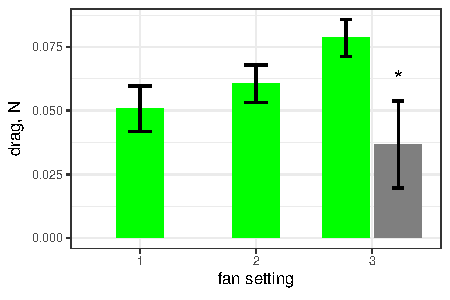
\includegraphics{data/results1.pdf}
\end{center}
\caption{Drag (mean$\pm$sd) for grapefruit (green) and metal (gray) leaves at different fan speeds. The smaller model metal leaf has less drag than the actual grapefruit leaves because of smaller area (two-way ANOVA, $p<\num{1.67e-5}$, $n=5$).}
\label{fig:results1}
\end{figure}

\begin{figure}
\begin{center}
\includegraphics{data/results2.pdf}
\end{center}
\caption{Drag, normalized by area, (mean$\pm$sd) for grapefruit (green) and metal (gray) leaves at different fan speeds. Normalized by area, the rigid metal leaf has significantly more drag than the flexible grapefruit leaves at low speeds and at the highest speed (two-way ANOVA, $p<0.003$, $n=5$).}
\label{fig:results2}
\end{figure}


\section{Discussion}
Here discuss what your results mean. Are your hypotheses supported or not? Do you have an answer to your overall research question?

\section{Acknowledgements}

% References
\bibliography{smith.bib}

\clearpage
\appendix
\section{Detailed methods and results}
\label{app:A}
Add more detailed stuff here... 
\end{document}
